\documentclass{article}
\usepackage[utf8]{inputenc}
\usepackage{graphicx}
\usepackage{makeidx}
\usepackage{geometry}
\usepackage{float}
\usepackage{indentfirst}

\renewcommand{\contentsname}{Índice}
\geometry{a4paper,total = {150mm,250mm},left = {30mm}, top = {30mm}}
\makeindex
\graphicspath{ {./imagens/} }
\begin{document}
\begin{capa}
	\begin{center}
	\vspace*{1.0cm}
	\huge{Universidade do Minho}\\
	[1.0cm]
	
\includegraphics{logo.jpg}\\
	[1.5cm]
	\huge{\textbf{Redes de Computadores}}\\
	[0.5cm]
	\textsc{RC-TP2}\\
	\textsc{\normalsize{Mestrado Integrado em Engenharia Informática}}\\
	\textsc{\normalsize{3º Ano}}\\
	\textsc{\normalsize{Grupo 61}}\\
	[12.0cm]
	\end{center}
	\begin{flushleft}
	\textsc{Renato André Araújo Azevedo \textbf{\hspace*{130pt} A89547}}\\
	\textsc{Gonçalo Costa de Almeida \textbf{\hspace*{151pt} A88292}}\\
	\textsc{Maria Sofia Martinho Gonçalves Jordão Marques \textbf{\hspace*{30pt} A87963}}\\
	\end{flushleft}
\end{capa}

\newpage
\tableofcontents
\newpage

\section{Captura e análise de Tramas Ethernet}
\subsection{Ex1}
\textbf{Anote os endereços MAC de origem e de destino da trama capturada.}\\\par
Endereço origem: 18:56:80:25:3e:15\par
Endereço destino: 00:d0:03:ff::94:00
\begin{figure}[h]
	\centering
	\includegraphics[scale = 0.8]{endereços-mac-ex1.JPG}
	\caption{Endereços MAC}
\end{figure}

\subsection{Ex2}
\textbf{Identifique a que sistemas se referem. Justifique.}\\\par
Uma vez que os endereços MAC correspondem a nós imediatamente adjacentes na rede, então o endereço destino corresponde ao router à qual estamos ligados, enquanto que o endereço origem corresponde à nossa máquina nativa.

\subsection{Ex3}
\textbf{Qual o valor hexadecimal do campo Type da trama Ethernet? O que significa?}\\\par
O valor hexadecimal do campo \texit{Type} é 0x800, e indica o tipo do protocolo encapsulado, neste caso, IPv4.
\begin{figure}[h]
	\centering
	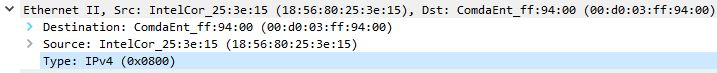
\includegraphics[scale = 0.8]{campo-type-ex3.JPG}
	\caption{Valor do campo Type}
\end{figure}

\subsection{Ex4}
\textbf{Quantos bytes são usados desde o início da trama até ao caractere ASCII “G” do método HTTP GET? Calcule e indique, em percentagem, a sobrecarga (overhead) introduzida pela pilha protocolar no envio do HTTP GET.}\\\par
Desde o início da trama até ao caractere ASCII “G” são usados 54 bytes. Como o tamanho total da trama é de 513 bytes, então o overhead introduzido pela pilha protocular é igual a 54/513 = 0.105263, o que corresponde a cerca de 10\% do tamanho total.
\newpage
\begin{figure}[h]
	\centering
	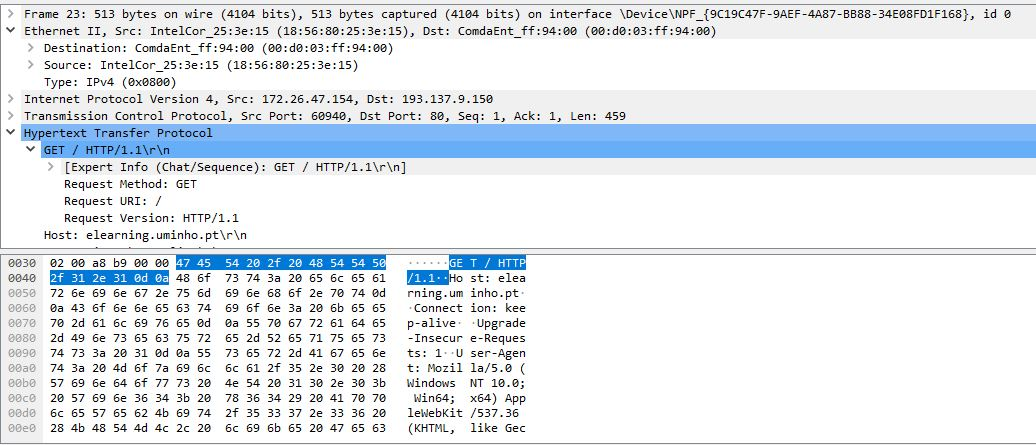
\includegraphics[scale = 0.5]{tamanho-mensagem-ex4.JPG}
	\caption{Trama capturada}
\end{figure} 

\subsection{Ex5}
\textbf{Através de visualização direta ou construindo um filtro específico, verifique se foram detetadas tramas com erros (por verificação do campo FCS (Frame Check Sequence)).}\\\par
Aplicando o filtro fcs, que mostra as tramas com erros, nenhum resultado é mostrado, o que significa que não foi detetada nenhuma trama com erros. 
\begin{figure}[h]
	\centering
	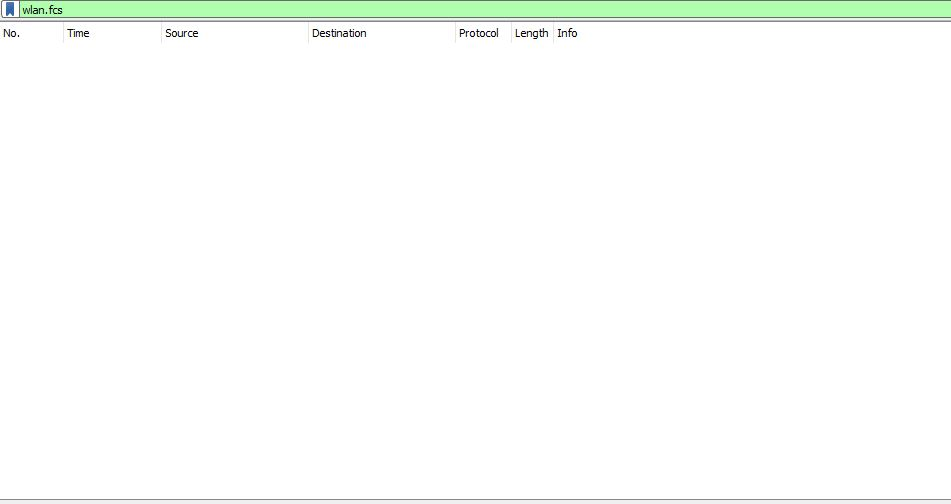
\includegraphics[scale = 0.4]{tramas-com-erros.JPG}
	\caption{Tramas com erros}
\end{figure}

\subsection{Ex6}
\textbf{Qual é o endereço Ethernet da fonte? A que sistema de rede corresponde? Justifique.}\\\par
O endereço \texit{Ethernet} da fonte é 00:d0:03:ff::94:00. Este endereço corresponde à rede a que estamos ligados, uma vez que estes endereços nós adjacentes numa mesma rede.
\begin{figure}[h]
	\centering
	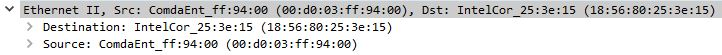
\includegraphics[scale = 0.8]{ex6.JPG}
	\caption{Endereços fonte e destino}
\end{figure}

\subsection{Ex7}
\textbf{Qual é o endereço MAC do destino? A que sistema corresponde?}\\\par
O endereço MAC do destino é 18:56:80:25:3e:15, e corresponde à nossa maquina nativa.

\subsection{Ex8}
\textbf{Atendendo ao conceito de desencapsulamento protocolar, identifique os vários protocolos contidos na trama recebida.}\\\par
\begin{figure}[h]
	\centering
	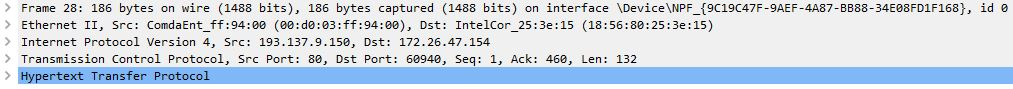
\includegraphics[scale = 0.6]{ex-8.JPG}
	\caption{Endereços fonte e destino}
\end{figure}
Os protocolos contidos na trama são Ethernet, IPv4 (Internet Protocol Version 4), TCP (Transmission Control Protocol), e HTTP (Hypertext Transfer Protocol).

\section{Protocolo ARP}
\subsection{Ex9}
\textbf{Observe o conteúdo da tabela ARP. Diga o que significa cada uma das colunas.}\\\par
A primeira coluna identifica os endereços ip, a segunda coluna representa os endereços MAC correspondentes, e a terceira coluna diz-nos o tipo de endereçamento. É ainda possivel verificar qual a interface onde os endereços estão definidos.
\begin{figure}[h]
	\centering
	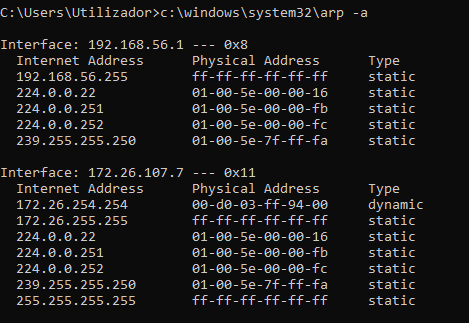
\includegraphics[scale = 0.8]{ex9.PNG}
	\caption{Endereços MAC}
\end{figure}

\subsection{Ex10}
\textbf{Qual é o valor hexadecimal dos endereços origem e destino na trama Ethernet que contém a mensagem com o pedido ARP (ARP Request)? Como interpreta e justifica o endereço destino usado?}\\\par
O endereço de origem é 68:94:23:a1:b2:a8.\par
O endereço de destino é ff:ff:ff:ff:ff:ff.\par
De forma a que o pedido ARP seja enviado para todas as máquinas da rede, este é enviado por broadcast, possuindo assim o endereço destino ff:ff:ff:ff:ff:ff, que corresponde a encaminhar a mensagem para todas as interfaces da rede local. Assim, a máquina que possuir o endereço pedido, devolverá uma resposta com o seu endereço MAC, e todas as outras irão ignorar a mensagem.
\begin{figure}[h]
	\centering
	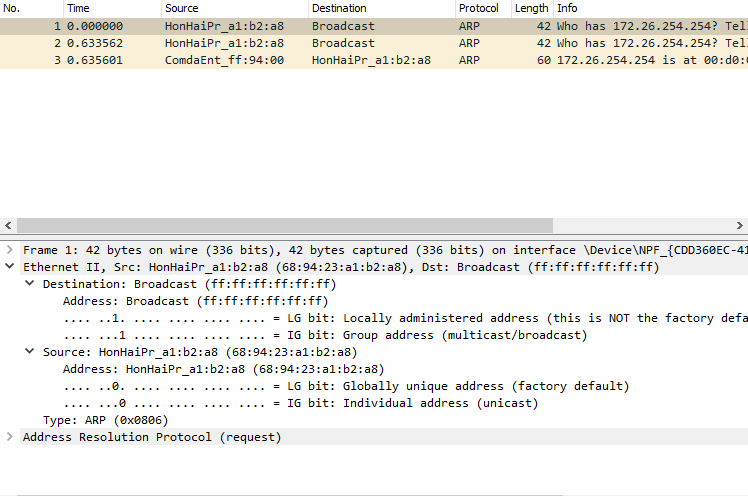
\includegraphics[scale = 0.43]{ex10.PNG}
	\caption{Endereços origem e destino}
\end{figure}

\subsection{Ex11}
\textbf{Qual o valor hexadecimal do campo tipo da trama Ethernet? O que indica?}\\\par
O campo tipo tem o valor hexadecimal 0x0806 (Type: ARP (0x0806)) e indica que o tipo de trama que estamos a tratar é de facto ARP.

\subsection{Ex12}
\textbf{Como pode confirmar que se trata efetivamente de um pedido ARP? Identifique que tipo de endereços estão contidos na mensagem ARP? Que conclui?}\\\par
O campo \textit{Type}, como observamos na questão anterior, diz-nos que estamos a tratar do protocolo ARP.\par
Os endereços que estão contidos na mensagem são endereços MAC e IP como podemos verificar no campo do address resolution protocol (request).
Podemos concluir de acordo com a figura que, o host cujo ip é 172.26.107.7 quer saber qual é o o endereço mac do host 172.26.254.254, então através da mensagem arp vai ser possivel determinar qual esse endereço. Assim, será possível associar, tanto na fonte como no destino, o endereço ip ao endereço mac.

\begin{figure}[h]
	\centering
	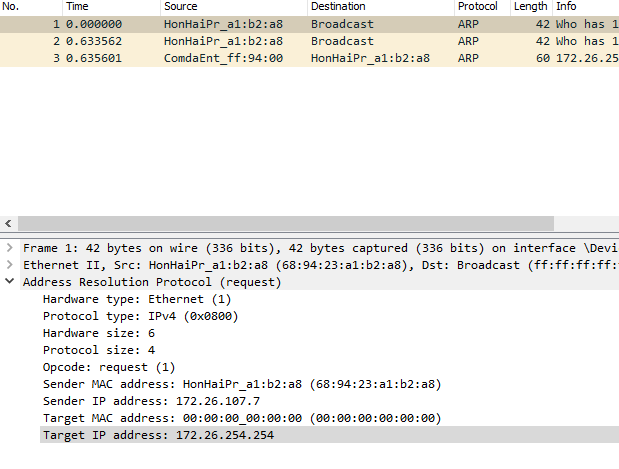
\includegraphics[scale = 0.5]{ex12.PNG}
	\caption{Endereços na mensagem ARP}
\end{figure}

\subsection{Ex13}
\textbf{Explicite que tipo de pedido ou pergunta é feita pelo host de origem?}\\\par
A pergunta feita é ''Who has 172.26.254.254? Tell 172.26.107.7''. Como podemos observar, perguntamos ao host qual é o enderço mac do host cujo ip é 172.26.254.254, que é o endereço à qual fizemos ping, e pedimos para que devolva a resposta ao host 172.26.107.7, que corresponde ao ip da nossa maquina.

\begin{figure}[h]
	\centering
	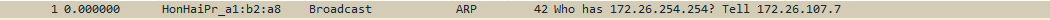
\includegraphics[scale = 0.54]{ex13.PNG}
	\caption{Endereços na mensagem ARP}
\end{figure}

\subsection{Ex14}
\textbf{Localize a mensagem ARP que é a resposta ao pedido ARP efetuado.}\\\par

\begin{figure}[h]
	\centering
	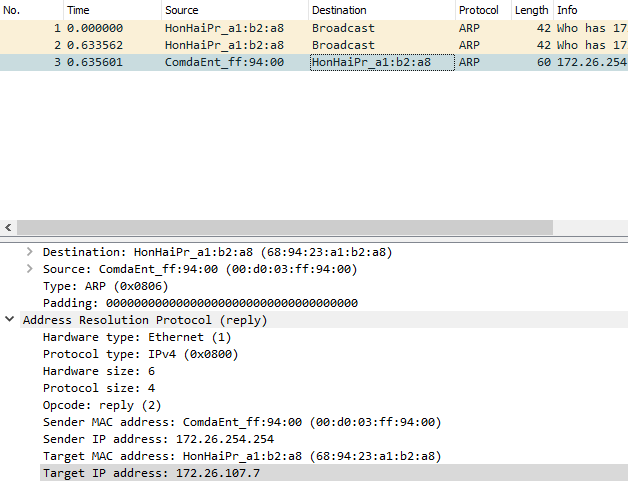
\includegraphics[scale = 0.6]{ex14.PNG}
	\caption{Endereços na mensagem ARP}
\end{figure}

\subsubsection{Alinea a}
\textbf{Qual o valor do campo ARP opcode? O que especifica?}\\\par
O valor do campo ARP opcode é: reply (2), e especifica que é uma resposta obtida ao ARP request feito anteriormente.

\subsubsection{Alinea b}
\textbf{Em que posição da mensagem ARP está a resposta ao pedido ARP?}\\\par
No campo Address Resolution Protocol (reply), podemos ver então que o endereço mac do host 172.26.254.254 é 00:d0:03:ff:94:00, ou seja a resposta é dada na campo \textit{Sender MAC address}.

\section{ARP Gratuito}
\subsection{Ex15}
\textbf{Identifique um pacote de pedido ARP gratuito originado pelo seu sistema. Analise o conteúdo de um pedido ARP gratuito e identifique em que se distingue dos restantes pedidos ARP. Registe a trama Ethernet correspondente. Qual o resultado esperado face ao pedido ARP gratuito enviado?}\\\par

\begin{figure}[h]
	\centering
	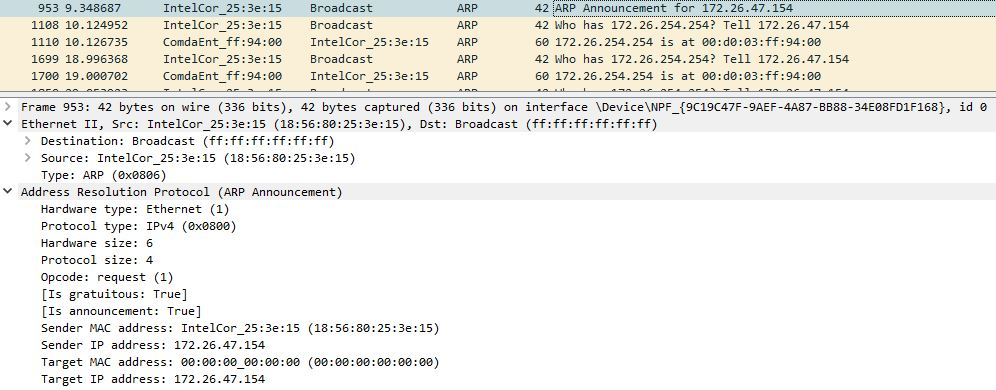
\includegraphics[scale = 0.6]{ex-15.png}
	\caption{ARP gratuito}
\end{figure}


Ao contrario dos restantes pedidos ARP, o ARP gratuito possui tanto no ip de origem como no ip destino, o ip da nossa maquina. Além disso, este pacote possui uma flag propria que o identifica como uma ARP gratuito. Este pedido ARP gratuito serve para informar à rede do ip da nossa máquina, bem como o endereço MAC. Tal como seria de esperar, neste pedido não é esperado uma resposta.

\section{Domínios de colisão}
\subsection{Ex16}
\begin{figure}[h]
	\centering
	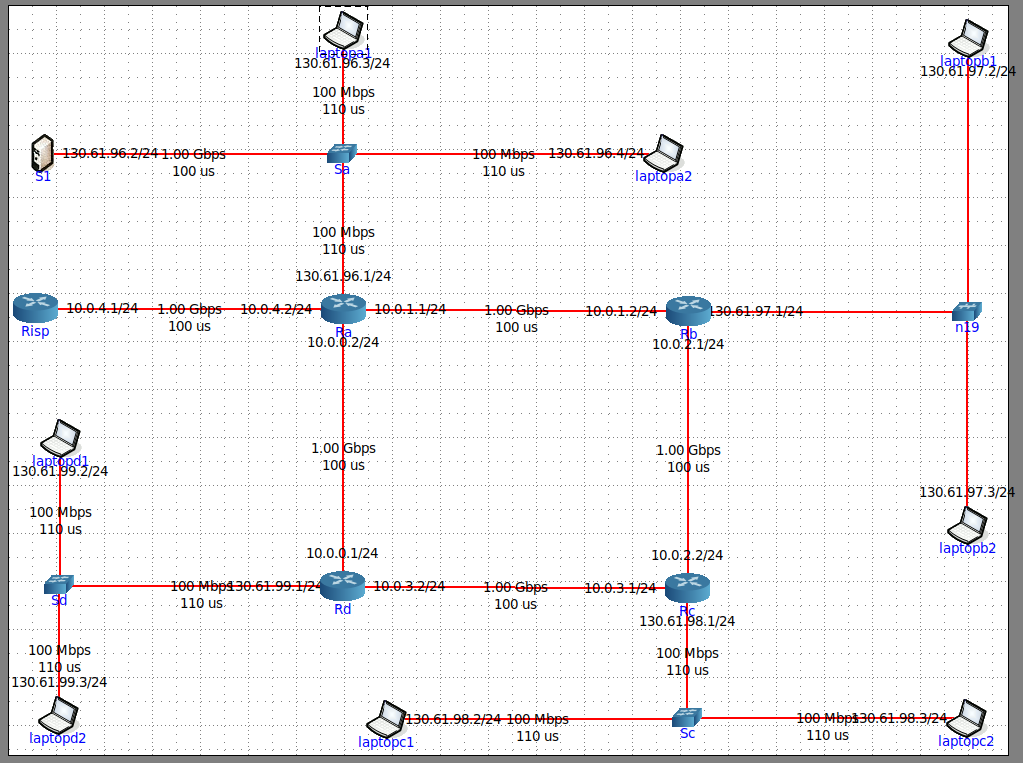
\includegraphics[scale = 0.3]{rede-ex16.PNG}
	\caption{Topologia}
\end{figure}

\textbf{Através da opção tcpdump verifique e compare como flui o tráfego nas diversas interfaces dos vários dispositivos no departamento A (LAN comutada) e no departamento B (LAN partilhada) quando gera tráfego intra-departamento (por exemplo, através do comando ping). Que conclui? Comente os resultados obtidos quanto à utilização de hubs e switches no contexto de controlar ou dividir domínios de colisão. Documente as suas observações e conclusões com base no tráfego observado/capturado.}\\\par
Ao fazer ping do laptop 1 para o laptop 2 no departamento A, podemos observar com o tcpdum (aberto no laptop 2 e no router) que apenas o laptop 2, e mais nenhuma outra interface da rede, irá receber a mensagem. Já no departamento B, isto não acontece, uma vez que ao dar ping do laptop 1 para o laptop 2, conseguimos verificar com o tcpdum que a mensagem chega até ao router. Estes resultados mostram que ao contrario do hub, o switch envia a mensagem apenas para o destino, enquanto que o hub faz broadcast da mensagem. Em termos de controlar ou dividir dominios de colisão, podemos concluir que os switch permitem um maior controlo, havendo uma separação dos domínios de colisão.

\newpage
\begin{figure}[h]
	\centering
	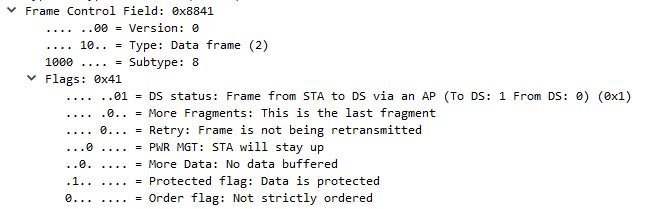
\includegraphics[scale = 0.3]{ex-16.PNG}
	\caption{Resultados}
\end{figure}

\section{Conclusão}
A realização deste trabalho prático permite um melhor entendimento do endereçamento ethernet e do protocolo ARP, bem como os seus diferentes campos. Além disso, percebemos melhor como funcionam os pedidos ARP numa rede, como por exemplo a existencia de ARPs gratuitos, e o seu proposito, bem como a importancia deste protocolo para as redes locais. Por fim, conseguimos ainda diferenciar um hub de um switch, com um melhor entendimento dos domínios de colisão, e como estes dois os tratam.

\printindex
\end{document}
